\chapter{الخلايا الكهروكيميائية والتحليل الكهربائي}\label{ch:g12:cells-and-electrolysis}

يُظهر هاتف 1 \% في مساء شتوي ثم ينطفئ. فإذا وُصل بالشاحن طوال الليل،
امتلأ من جديد في الصباح. ففي بطاريته يجري \omterm{def:g7:chemical-reactions:reaction}{التفاعل الكيميائي} نفسه
في اتجاه خلال النهار، فيعطي طاقة كهربائية، ويُدفع
في الاتجاه الآخر ليلًا بالشاحن. ويصير \omterm{def:g11:redox:reaction}{تفاعل الأكسدة والاختزال} مصدرًا
للكهرباء حين تُجبر إلكتروناته على الانتقال عبر سلك؛
والكهرباء، إذا دُفعت عبر \omterm{def:g2:mixing-and-dissolving:dissolve}{محلول}، يمكنها أن تفرض \omterm{def:g11:redox:reaction}{تفاعل أكسدة واختزال}
لا يحدث من تلقاء نفسه أبدًا.

\begin{recall}
المؤكسدات تكتسب \omterm{def:g9:inside-the-atom:nucleus}{الإلكترونات}، والمختزلات تفقدها؛ وأنصاف المعادلات، ومزدوجات
\omterm{def:g11:redox:oxidation}{الأكسدة} \omterm{def:g11:redox:oxidation}{والاختزال} وتفاعلاتها (\cref{ch:g11:redox}). وتتطور المجموعة حتى
$Q = K$ (\cref{ch:g12:equilibrium}). ومحاليل \omterm{def:g9:ions:ion}{الأيونات} توصل
(\cref{ch:g9:ions})؛ \omterm{def:g10:the-mole:amount}{والمول} \omterm{def:g10:the-mole:avogadro}{وثابت أفوغادرو}
(\cref{ch:g10:the-mole}).
\end{recall}

\begin{omfigure}
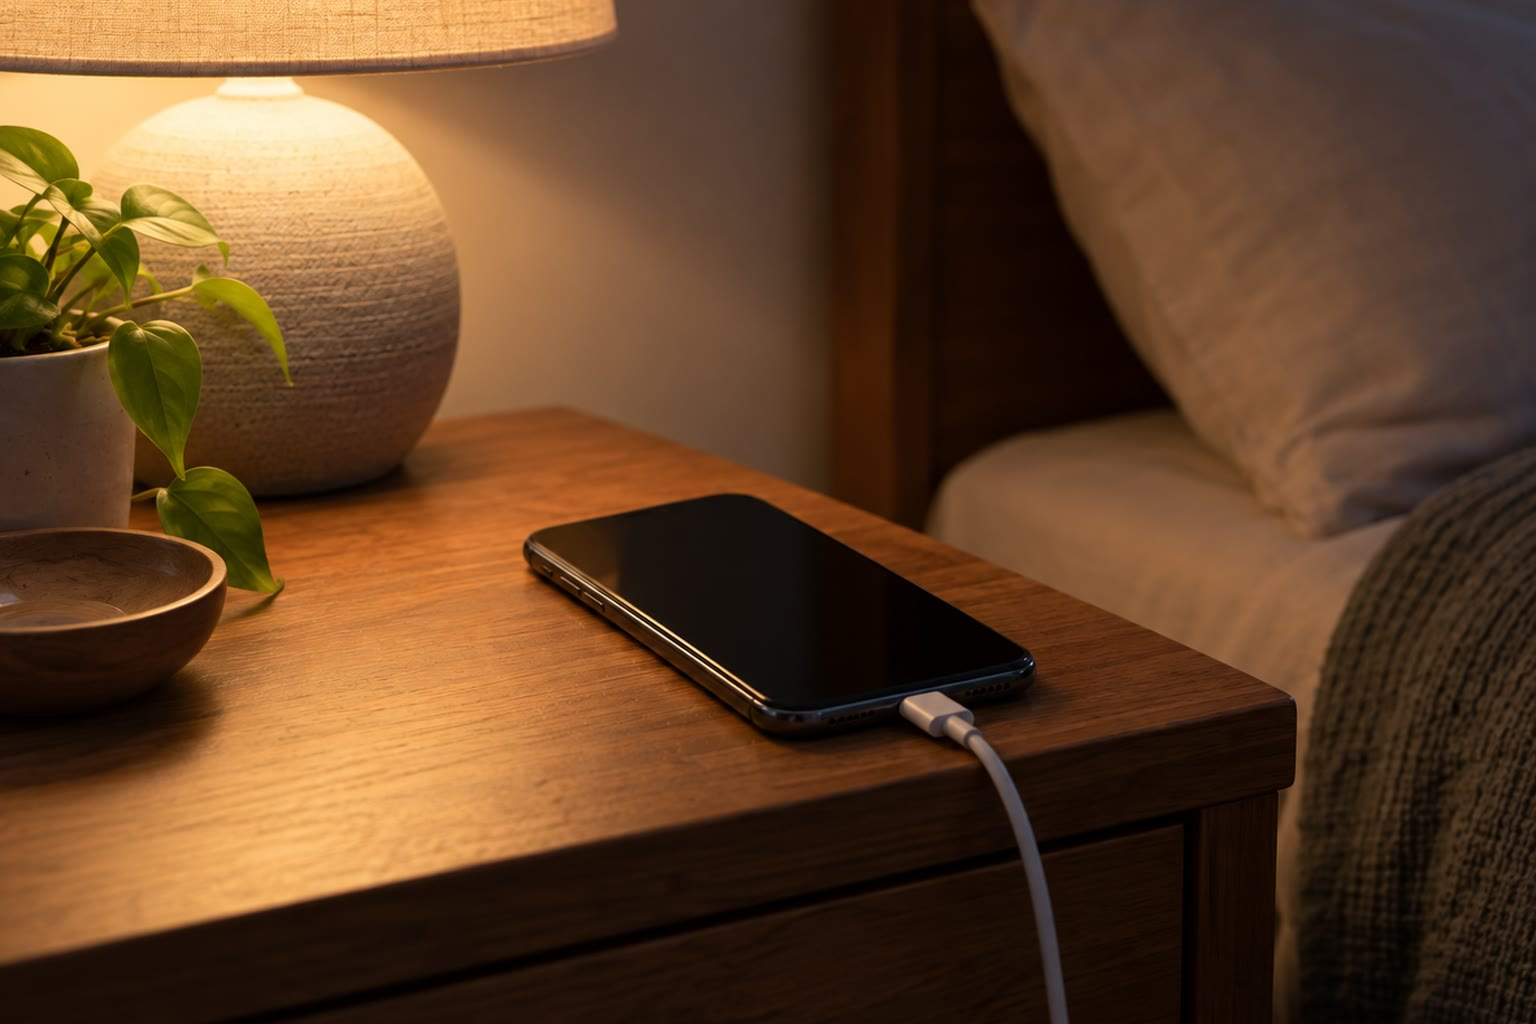
\includegraphics[width=0.45\linewidth]{images/book1/ai/g12-phone-charging.jpg}

{\small شحن هاتف: تفاعل يُدفع في الاتجاه المعاكس طوال الليل.}
\end{omfigure}

\section{تفاعل أكسدة واختزال مقسوم نصفين}

حين تُغمس صفيحة خارصين في \omterm{def:g2:mixing-and-dissolving:dissolve}{محلول} كبريتات النحاس، يتأكسد الخارصين
وتُختزل \omterm{def:g9:ions:ion}{أيونات} النحاس عند سطح الصفيحة،
\ce{Zn + Cu^{2+} -> Zn^{2+} + Cu}: فتنتقل \omterm{def:g9:inside-the-atom:nucleus}{الإلكترونات} مباشرة من \omterm{def:g9:periodic-table-first-look:metal}{الفلز}
إلى \omterm{def:g9:ions:ion}{الأيونات}، وتضيع الطاقة على هيئة قليل من الحرارة. فافصل
النصفين، وصِل بينهما بسلك: فيجب على \omterm{def:g9:inside-the-atom:nucleus}{الإلكترونات} الآن أن تنتقل عبر
السلك، ويمكنها أن تضيء مصباحًا في طريقها.

\begin{definition}[الخلية الكهروكيميائية، نصف الخلية، الجسر الملحي]\label{def:g12:cells-and-electrolysis:cell}
\emph{الخلية الكهروكيميائية}\index{خلية كهروكيميائية} تنتج
طاقة كهربائية من \omterm{def:g11:redox:reaction}{تفاعل أكسدة واختزال} تجري أكسدته واختزاله
في حجرتين منفصلتين. وكل حجرة، أي قطب فلزي
مغموس في \omterm{def:g2:mixing-and-dissolving:dissolve}{محلول} أيوناته، هي
\emph{نصف خلية}\index{نصف خلية}. و\emph{الجسر الملحي}\index{جسر ملحي}،
وهو أنبوب أو شريط ورقي مشبع \omterm{def:g2:mixing-and-dissolving:dissolve}{بمحلول} \omterm{def:g9:ions:ion}{أيونات}، يصل بين
المحلولين ويغلق الدارة مع إبقائهما منفصلين.
\end{definition}

\begin{definition}[المصعد، المهبط]\label{def:g12:cells-and-electrolysis:anode}
القطب الذي تجري عنده \omterm{def:g11:redox:oxidation}{الأكسدة} هو
\emph{المصعد}\index{مصعد}؛ والقطب الذي يجري عنده \omterm{def:g11:redox:oxidation}{الاختزال}
هو \emph{المهبط}\index{مهبط}.
\end{definition}

\begin{omfigure}
\begin{tikzpicture}[font=\small, scale=1.25]
  \pic[transform shape] at (0,0) {beaker={0.7}{black!6}};
  \pic[transform shape] at (4,0) {beaker={0.7}{cyan!70!blue!35}};
  \pic[transform shape] (zn) at (-0.3,0.25) {electrode={black!30}};
  \pic[transform shape] (cu) at (4.3,0.25) {electrode={orange!70!brown}};
  \pic[transform shape] at (0.35,0.6) {saltbridge={3.3}};
  \pic[transform shape] (v) at (2,3.9) {meter={1.10 V}};
  \draw[black!70, thick] (zn-top) |- (1.0,3.4) -| (v-a);
  \draw[black!70, thick] (cu-top) |- (3.0,3.4) -| (v-b);
  \draw[->, omProp, very thick] (0.2,3.55) -- (1.0,3.55);
  \draw[->, omProp, very thick] (3.0,3.55) -- (3.8,3.55);
  \node[omProp, font=\footnotesize] at (0.6,3.75) {$e^-$};
  \node[omProp, font=\footnotesize] at (3.4,3.75) {$e^-$};
  \node[anchor=north, align=center] at (-0.2,-0.15) {\foreignlanguage{arabic}{المصعد \babelsublr{($-$)}: الخارصين}\\ \ce{Zn -> Zn^{2+} + 2e-}};
  \node[anchor=north, align=center] at (4.2,-0.15) {\foreignlanguage{arabic}{المهبط \babelsublr{($+$)}: النحاس}\\ \ce{Cu^{2+} + 2e- -> Cu}};
  \node[font=\footnotesize, anchor=east, align=right] at (-0.95,0.7) {\ce{Zn^{2+}}\\ \ce{SO4^{2-}}};
  \node[font=\footnotesize, anchor=west, align=left] at (4.95,0.7) {\ce{Cu^{2+}}\\ \ce{SO4^{2-}}};
  \node[font=\footnotesize, align=center] at (2,2.45) {الجسر الملحي\\ (\foreignlanguage{arabic}{\ce{K+}، \ce{NO3-}})};
\end{tikzpicture}

{\small خلية دانيال. تغادر \omterm{def:g9:inside-the-atom:nucleus}{الإلكترونات} \omterm{def:g12:cells-and-electrolysis:anode}{مصعد} الخارصين عبر
السلك وتدخل \omterm{def:g12:cells-and-electrolysis:anode}{مهبط} النحاس؛ وفي \omterm{def:g12:cells-and-electrolysis:cell}{الجسر الملحي} تتحرك \omterm{def:g9:ions:ion}{الأيونات} لتحفظ
كل \omterm{def:g2:mixing-and-dissolving:dissolve}{محلول} متعادلًا.}
\end{omfigure}

\begin{proposition}[إلى أين تذهب الإلكترونات]\label{prop:g12:cells-and-electrolysis:flow}
في خلية تولّد تيارًا، تغادر \omterm{def:g9:inside-the-atom:nucleus}{الإلكترونات} الخلية من \omterm{def:g12:cells-and-electrolysis:anode}{المصعد}،
حيث تحررها \omterm{def:g11:redox:oxidation}{الأكسدة}، وتنتقل عبر الدارة
الخارجية، وتدخل من \omterm{def:g12:cells-and-electrolysis:anode}{المهبط}، حيث يأخذها
\omterm{def:g11:redox:oxidation}{الاختزال}. \omterm{def:g12:cells-and-electrolysis:anode}{فالمصعد} هو القطب السالب، \omterm{def:g12:cells-and-electrolysis:anode}{والمهبط} القطب
الموجب. وفي الداخل تحمل \omterm{def:g9:ions:ion}{الأيونات} التيار: فتتحرك الكاتيونات نحو
\omterm{def:g12:cells-and-electrolysis:anode}{المهبط}، والأنيونات نحو \omterm{def:g12:cells-and-electrolysis:anode}{المصعد}.
\end{proposition}

\begin{proof}
تنتج \omterm{def:g11:redox:oxidation}{الأكسدة} \omterm{def:g9:inside-the-atom:nucleus}{الإلكترونات} عند \omterm{def:g12:cells-and-electrolysis:anode}{المصعد}؛ ويستهلكها \omterm{def:g11:redox:oxidation}{الاختزال}
عند \omterm{def:g12:cells-and-electrolysis:anode}{المهبط}؛ والسلك هو الطريق الوحيد بينهما. ولولا \omterm{def:g9:ions:ion}{أيونات} الجسر
لصار كل \omterm{def:g2:mixing-and-dissolving:dissolve}{محلول} مشحونًا، وهي تمنع
ذلك.
\end{proof}

\begin{method}[وصف خلية]\label{met:g12:cells-and-electrolysis:describe}
\begin{enumerate}
  \item اكتب \omterm{def:g11:redox:reaction}{تفاعل الأكسدة والاختزال} الإجمالي الذي يجري تلقائيًا.
  \item قسّمه إلى نصفي معادلتين: \omterm{def:g11:redox:oxidation}{الأكسدة} (\omterm{def:g12:cells-and-electrolysis:anode}{المصعد})
        \omterm{def:g11:redox:oxidation}{والاختزال} (\omterm{def:g12:cells-and-electrolysis:anode}{المهبط}).
  \item عيّن القطبية: \omterm{def:g12:cells-and-electrolysis:anode}{المصعد} $-$، \omterm{def:g12:cells-and-electrolysis:anode}{والمهبط} $+$؛ واتجاه
        \omterm{def:g9:inside-the-atom:nucleus}{الإلكترونات} في السلك (من \omterm{def:g12:cells-and-electrolysis:anode}{المصعد} إلى \omterm{def:g12:cells-and-electrolysis:anode}{المهبط}) واتجاه التيار
        (من \omterm{def:g12:cells-and-electrolysis:anode}{المهبط} إلى \omterm{def:g12:cells-and-electrolysis:anode}{المصعد}).
  \item صف حركة \omterm{def:g9:ions:ion}{الأيونات} في الجسر.
\end{enumerate}
\end{method}


\begin{history}[عمود فولتا، 1800]
في سنة 1800 رصّ الفيزيائي أليساندرو فولتا أقراصًا من فلزين
مختلفين، الخارصين والنحاس أو الفضة، تفصل بينها قطع من القماش مبللة
بالماء المالح، فحصل على تيار كهربائي مستمر: أول بطارية. وقد
أعطت الفيزيائيين أول مصدر متواصل للكهرباء، وأعطت
الكيميائيين أداة جديدة: ففي غضون سنوات قليلة أتاح \omterm{def:g12:cells-and-electrolysis:electrolysis}{التحليل الكهربائي} فصل الصوديوم
والبوتاسيوم أول مرة.
\end{history}

\begin{omfigure}
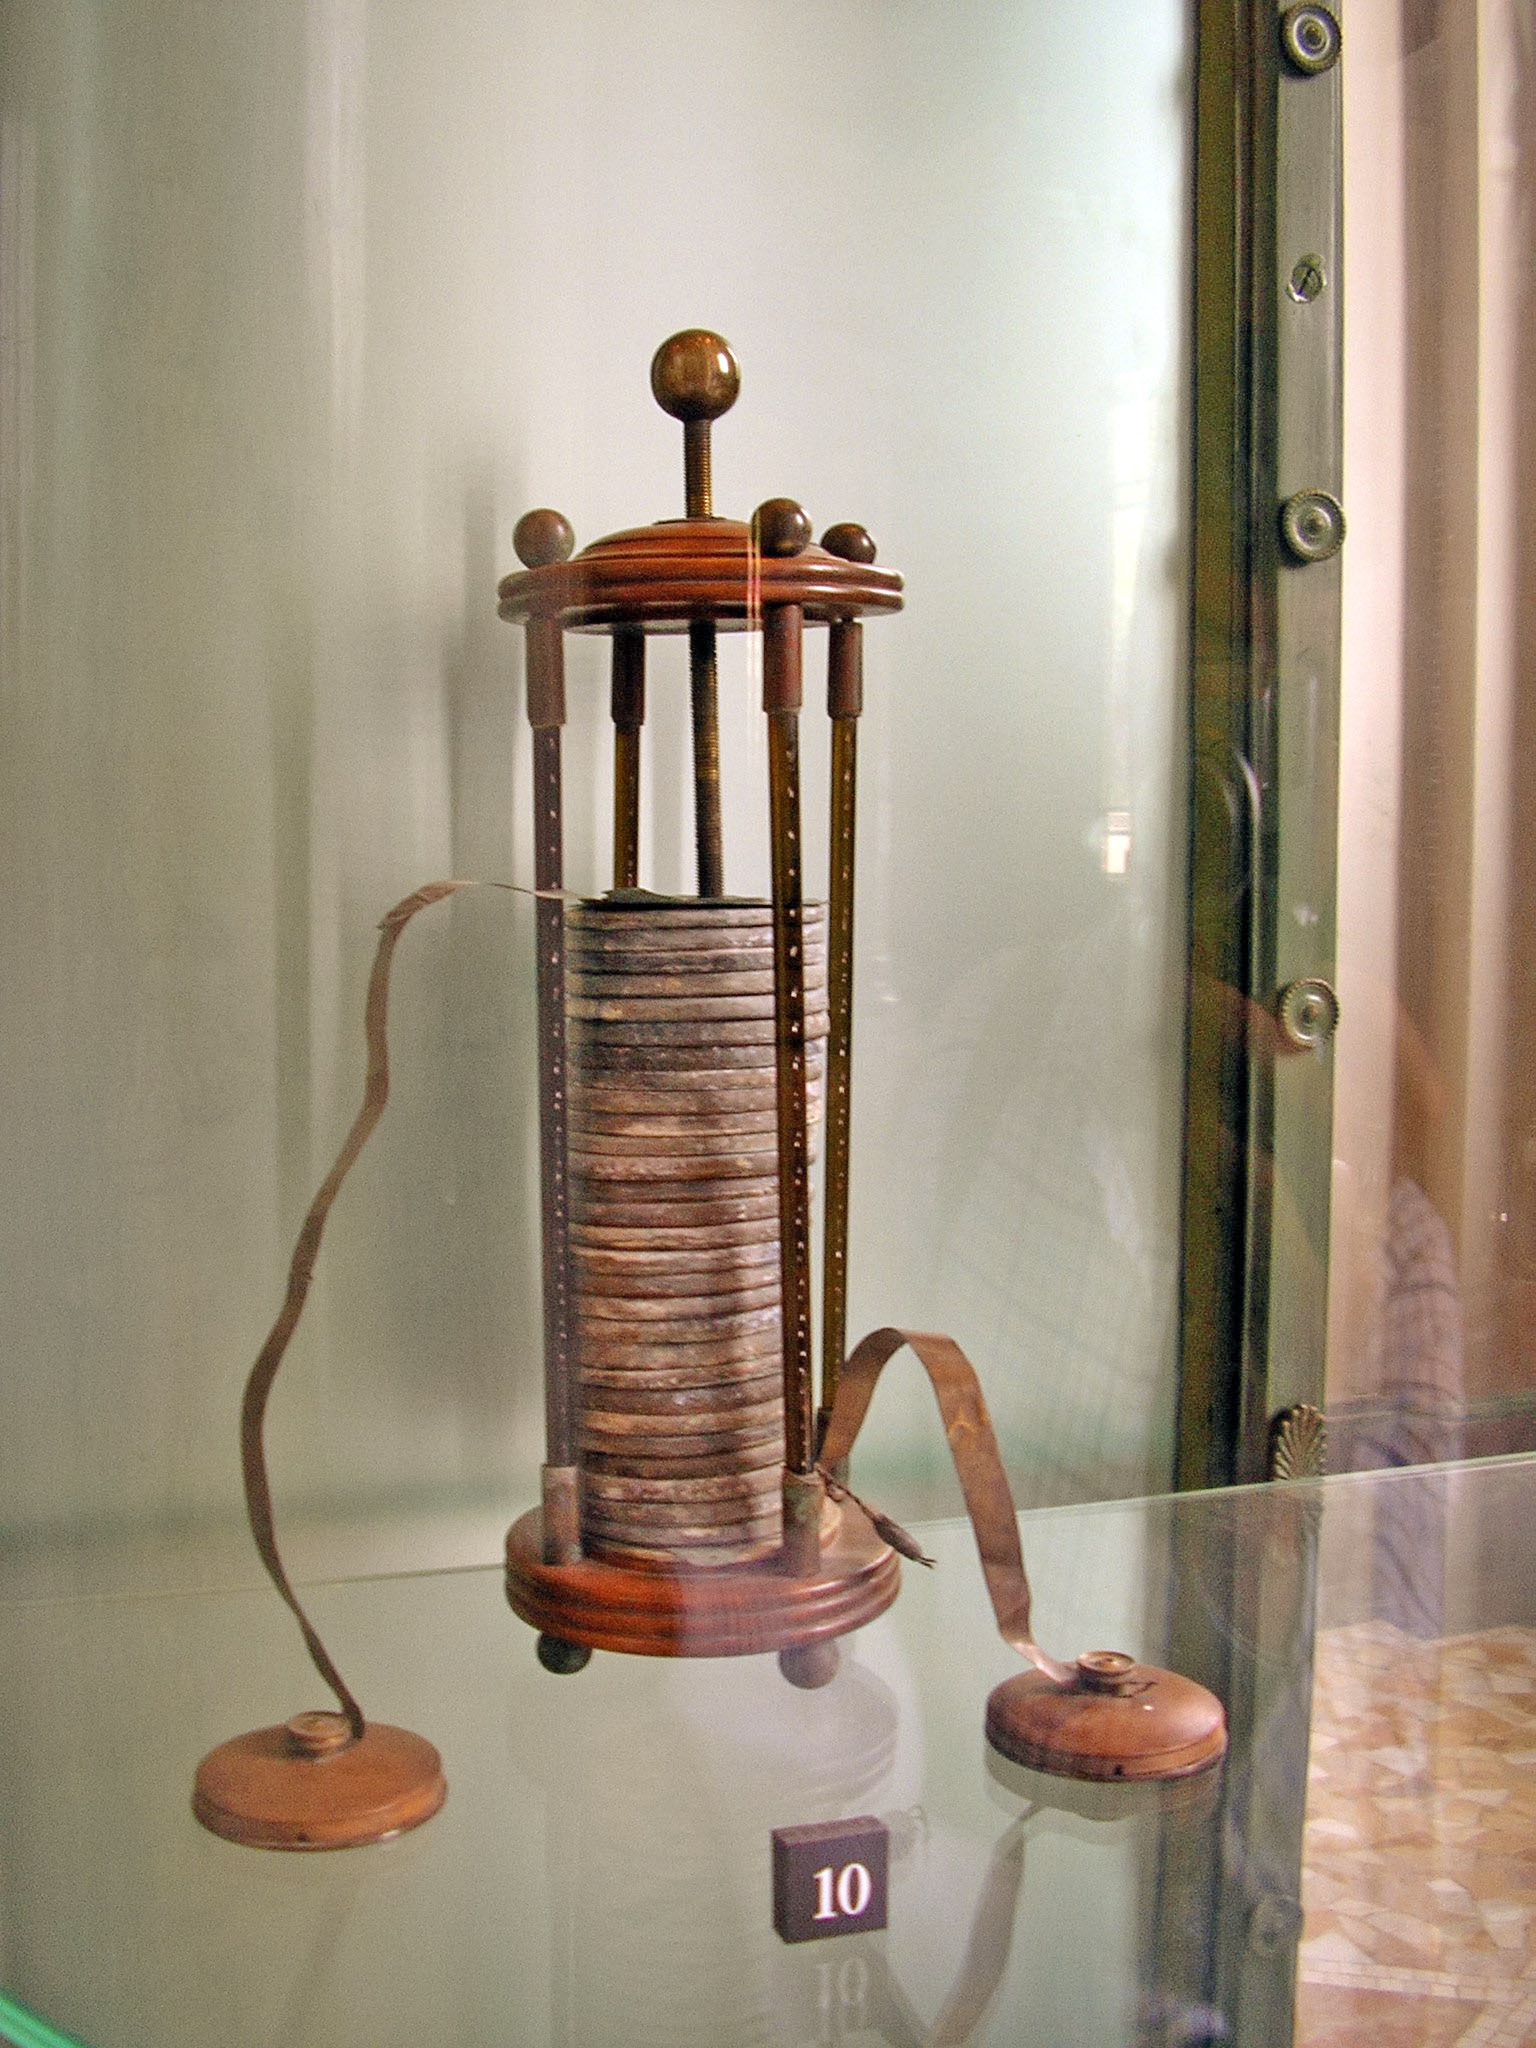
\includegraphics[width=0.24\linewidth]{images/book1/volta-pile.jpg}

{\small عمود فولتا في متحف. تصوير GuidoB، CC BY-SA 3.0.}
\end{omfigure}

\section{جهد الخلية}

\begin{definition}[جهد الخلية]\label{def:g12:cells-and-electrolysis:emf}
\emph{جهد الخلية}\index{جهد الخلية} هو التوتر المقيس
بين قطبي خلية لا تولّد تيارًا (دارة مفتوحة)،
بمقياس فولت؛ ويكون موجبًا حين يكون القطب الموجب لمقياس الفولت
على \omterm{def:g12:cells-and-electrolysis:anode}{المهبط}.
\end{definition}

\begin{example}[خلية دانيال]\label{ex:g12:cells-and-electrolysis:daniell}
% ledger: e0:Cu, e0:Zn, emf:Daniell
حين يكون تركيز المحلولين كليهما \qty{1}{mol/L}، تعطي خلية دانيال
\qty{1.10}{V}. أما كيف يُتنبأ بهذا الجهد من جداول جهود
الأقطاب فيبيّنه مجلد السنة الأولى.
\end{example}

\begin{remark}[لماذا تنفد الخلية]\label{rem:g12:cells-and-electrolysis:runs-down}
لتفاعل الخلية، \ce{Zn + Cu^{2+} -> Zn^{2+} + Cu}، ثابت $K$ كبير
جدًا. وبينما تعمل الخلية، يزداد $Q = [\ce{Zn^{2+}}]/[\ce{Cu^{2+}}]$،
ويستمر التفاعل ما دام $Q < K$. فإذا نفد
أحد المتفاعلين (الخارصين، أو \omterm{def:g9:ions:ion}{أيونات} النحاس)، توقف التيار: فتكون
الخلية «فارغة».
\end{remark}

\section{الشحنة والسعة}

\begin{definition}[ثابت فاراداي، السعة]\label{def:g12:cells-and-electrolysis:capacity}
\emph{ثابت فاراداي}\index{ثابت فاراداي} $F$ هو الشحنة
الكهربائية \omterm{def:g10:the-mole:amount}{لمول} واحد من \omterm{def:g9:inside-the-atom:nucleus}{الإلكترونات}، $F = N_A e = \qty{96485}{C/mol}$.
و\emph{سعة}\index{سعة} الخلية هي أكبر شحنة كهربائية
تستطيع توليدها، وكثيرًا ما تُعطى بالأمبير ساعة: $\qty{1}{A.h} = \qty{3600}{C}$.
\end{definition}

\begin{proposition}[الشحنة وكمية الإلكترونات]\label{prop:g12:cells-and-electrolysis:charge}
% ledger: const:F, const:NA, const:e
تيار شدته $I$ يسري مدة $\Delta t$ ينقل الشحنة
$Q = I\,\Delta t$، أي كمية من \omterm{def:g9:inside-the-atom:nucleus}{الإلكترونات}
\[
  n(e^-) = \frac{Q}{F} = \frac{I\,\Delta t}{F} .
\]
\end{proposition}

\begin{proof}
كل \omterm{def:g9:inside-the-atom:nucleus}{إلكترون} يحمل الشحنة الأولية $e$؛ و$n$ \omterm{def:g10:the-mole:amount}{مول} من \omterm{def:g9:inside-the-atom:nucleus}{الإلكترونات}
تحمل $n N_A e = n F$.
\end{proof}

\begin{example}[سعة خلية دانيال]\label{ex:g12:cells-and-electrolysis:capacity}
% ledger: aw:Zn, const:F
يحوي قطب الخارصين \qty{6.5}{g} من الخارصين القابل للتفاعل، أي
$6.5/65.4 = \qty{0.099}{mol}$. وكل \omterm{def:g7:atoms-and-molecules:atom}{ذرة} خارصين تعطي إلكترونين:
$n(e^-) = \qty{0.199}{mol}$، إذن $Q = 0.199 \times 96485 = \qty{1.9e4}{C}$،
أي نحو $\qty{1.9e4}{}/3600 = \qty{5.3}{A.h}$، إذا لم تنفد \omterm{def:g9:ions:ion}{أيونات}
النحاس قبل ذلك.
\end{example}

\section{التحليل الكهربائي}

\begin{definition}[التحليل الكهربائي، المركم]\label{def:g12:cells-and-electrolysis:electrolysis}
\emph{التحليل الكهربائي}\index{تحليل كهربائي} \omterm{def:g11:redox:reaction}{تفاعل أكسدة واختزال} يفرضه
مولّد كهربائي، في الاتجاه المعاكس للاتجاه الذي كان
سيأخذه من تلقاء نفسه. و\emph{المركم}\index{مركم} خلية
قابلة لإعادة الشحن: فأثناء الشحن يدفع المولّد تفاعلها
في الاتجاه المعاكس، كتحليل كهربائي.
\end{definition}

\begin{inthelab}[التحليل الكهربائي للماء]
يُغمس قطبان في ماء جُعل موصلًا بقليل من كبريتات
الصوديوم، كلٌّ منهما تحت أنبوب اختبار مقلوب مملوء \omterm{def:g2:mixing-and-dissolving:dissolve}{بالمحلول}. ومع
مولّد من بضعة فولتات، تصعد فقاعات من القطبين كليهما: عند
\omterm{def:g12:cells-and-electrolysis:anode}{المهبط} (الموصول بالقطب $-$) ثنائي الهيدروجين، وعند \omterm{def:g12:cells-and-electrolysis:anode}{المصعد}
ثنائي الأكسجين، والأول ضعف الثاني. فعود مشتعل
يفرقع في الغاز الأول؛ وعود متوهج يشتعل من جديد في الثاني.
\end{inthelab}

\begin{omfigure}
\begin{tikzpicture}[font=\small, scale=1.2]
  % a trough of water, two inverted tubes standing in it
  \fill[omWater] (-1.4,0) rectangle (1.4,1.1);
  \foreach \x/\g in {-0.6/1.2, 0.6/0.6} {
    \fill[omWater] (\x-0.18,0.3) rectangle (\x+0.18,2.9);
    \fill[white] (\x-0.18,{2.9-\g}) rectangle (\x+0.18,2.9);
    \fill[white] (\x,2.9) circle (0.18);
    \draw[om glass] (\x-0.18,0.3) -- (\x-0.18,2.9) arc[start angle=180, end angle=0, radius=0.18] -- (\x+0.18,0.3);
  }
  \draw[om glass] (-1.5,1.25) -- (-1.4,1.15) -- (-1.4,0) -- (1.4,0) -- (1.4,1.15) -- (1.5,1.25);
  \fill[black!55] (-0.65,0) rectangle (-0.55,0.6);
  \fill[black!55] (0.55,0) rectangle (0.65,0.6);
  \node[draw, fill=white, minimum width=1.6cm, minimum height=0.45cm, font=\footnotesize] (g) at (0,-0.75) {مولّد};
  \draw[black!70, thick] (-0.6,0) -- (-0.6,0 |- g.north);
  \draw[black!70, thick] (0.6,0) -- (0.6,0 |- g.north);
  \node[font=\footnotesize] at (-0.78,-0.3) {$-$};
  \node[font=\footnotesize] at (0.78,-0.3) {$+$};
  \node[anchor=east, align=right] at (-0.95,2.5) {ثنائي الهيدروجين\\ (المهبط)};
  \node[anchor=west, align=left] at (0.95,2.5) {ثنائي الأكسجين\\ (المصعد)};
\end{tikzpicture}

{\small \omterm{def:g12:cells-and-electrolysis:electrolysis}{التحليل الكهربائي} للماء: يتجمع فوق القطبين من ثنائي الهيدروجين ضعف
ما يتجمع من ثنائي الأكسجين.}
\end{omfigure}


\begin{example}[الماء مشطورًا]\label{ex:g12:cells-and-electrolysis:water}
عند \omterm{def:g12:cells-and-electrolysis:anode}{المهبط}: \ce{2H2O + 2e- -> H2 + 2OH-}؛ وعند \omterm{def:g12:cells-and-electrolysis:anode}{المصعد}:
\ce{6H2O -> O2 + 4H3O+ + 4e-}. ولكل أربعة \omterm{def:g9:inside-the-atom:nucleus}{إلكترونات}، جزيئان من
ثنائي الهيدروجين \omterm{def:g7:atoms-and-molecules:molecule}{وجزيء} من ثنائي الأكسجين، بينما تتحد \omterm{def:g9:ions:ion}{أيونات} \ce{H3O+} و\ce{OH-}
المتكوّنة عند القطبين من جديد ماءً: فالحصيلة
\ce{2H2O -> 2H2 + O2}، وهي
عكس \omterm{def:g4:what-a-fire-needs:burning}{احتراق} الهيدروجين، وتحتاج إلى طاقة كي تحدث.
\end{example}

\begin{method}[الكتلة المترسبة بالتحليل الكهربائي]\label{met:g12:cells-and-electrolysis:mass}
\begin{enumerate}
  \item اكتب \omterm{def:g11:redox:couple}{نصف المعادلة} عند القطب الذي يتكوّن عنده \omterm{def:g9:periodic-table-first-look:metal}{الفلز}،
        مثلًا \ce{Cu^{2+} + 2e- -> Cu}.
  \item احسب الشحنة $Q = I \Delta t$ و$n(e^-) = Q/F$.
  \item اقسم على عدد \omterm{def:g9:inside-the-atom:nucleus}{الإلكترونات} لكل \omterm{def:g7:atoms-and-molecules:atom}{ذرة}: $n(\ce{Cu}) =
        n(e^-)/2$؛ ثم $m = n \times M$.
\end{enumerate}
\end{method}


\begin{example}[تنقية النحاس]\label{ex:g12:cells-and-electrolysis:refining}
% ledger: aw:Cu, const:F
يُجعل النحاس غير النقي الآتي من المصهر مصعدًا لخلية \omterm{def:g12:cells-and-electrolysis:electrolysis}{تحليل كهربائي}
في \omterm{def:g2:mixing-and-dissolving:dissolve}{محلول} كبريتات النحاس، وصفيحة رقيقة من النحاس النقي مهبطًا.
فعند \omterm{def:g12:cells-and-electrolysis:anode}{المصعد} \omterm{def:g2:mixing-and-dissolving:dissolve}{يذوب} النحاس، \ce{Cu -> Cu^{2+} + 2e-}؛ وعند \omterm{def:g12:cells-and-electrolysis:anode}{المهبط}
يترسب النحاس النقي، \ce{Cu^{2+} + 2e- -> Cu}؛ والشوائب تسقط إلى
القاع أو تبقى في \omterm{def:g2:mixing-and-dissolving:dissolve}{المحلول}. وتيار شدته \qty{100}{A} مدة
\qty{24}{h} ينقل $Q = 100 \times 86400 = \qty{8.64e6}{C}$، أي
$n(e^-) = \qty{89.5}{mol}$، تُرسّب $89.5/2 = \qty{44.8}{mol}$ من
النحاس: \qty{2.84}{kg}.
\end{example}

\begin{omfigure}
\begin{tikzpicture}[font=\small, scale=1.25]
  \pic[transform shape] at (0,0) {beaker={0.75}{cyan!70!blue!35}};
  \pic[transform shape] (an) at (-0.4,0.2) {electrode={orange!40!brown!80!black}};
  \pic[transform shape] (ca) at (0.4,0.2) {electrode={orange!80!brown}};
  \foreach \p in {(-0.6,0.08),(-0.5,0.12),(-0.3,0.07),(-0.2,0.1)} \fill[black!55] \p circle (0.03);
  \node[draw, fill=white, font=\footnotesize, minimum width=1.6cm] (g) at (0,3.4) {مولّد};
  \draw[black!70, thick] (an-top) -- (an-top |- g.south);
  \draw[black!70, thick] (ca-top) -- (ca-top |- g.south);
  \node[font=\footnotesize] at (-0.58,2.95) {$+$};
  \node[font=\footnotesize] at (0.58,2.95) {$-$};
  \draw[omProp, thick, <-] (-0.55,1.2) -- (-1.6,1.6) node[left, align=right, text=black] {مصعد من نحاس\\ غير نقي: يذوب};
  \draw[omProp, thick, <-] (0.55,1.2) -- (1.6,1.6) node[right, align=left, text=black] {مهبط من نحاس\\ نقي: ينمو};
  \draw[omProp, thick, <-] (-0.35,0.1) -- (-1.6,0.3) node[left, text=black] {الشوائب};
\end{tikzpicture}

{\small تنقية النحاس \omterm{def:g12:cells-and-electrolysis:electrolysis}{بالتحليل الكهربائي}: ينتقل النحاس من \omterm{def:g12:cells-and-electrolysis:anode}{المصعد} غير النقي
إلى \omterm{def:g12:cells-and-electrolysis:anode}{المهبط} النقي عبر \omterm{def:g2:mixing-and-dissolving:dissolve}{المحلول}.}
\end{omfigure}

\section{البطاريات والمراكم وخلايا الوقود}

كل بطارية خلية، وكل بطارية قابلة لإعادة الشحن \omterm{def:g12:cells-and-electrolysis:electrolysis}{مركم}. ويعمل
\omterm{def:g12:cells-and-electrolysis:electrolysis}{مركم} الرصاص والحمض في السيارة بالرصاص وأكسيد الرصاص وحمض
الكبريتيك؛ ويحرّك \omterm{def:g12:cells-and-electrolysis:electrolysis}{مركم} \omterm{def:g9:ions:ion}{أيونات} الليثيوم في الهاتف \omterm{def:g9:ions:ion}{أيونات} الليثيوم بين
قطبين، أحدهما من الغرافيت والآخر من أكسيد فلزي، عبر إلكتروليت سائل
أو بوليمري، بينما تدور \omterm{def:g9:inside-the-atom:nucleus}{الإلكترونات} في الدارة
الخارجية. وخلية \omterm{def:g4:what-a-fire-needs:fuel}{الوقود} خلية تُغذّى بمتفاعلاتها باستمرار:
فخلية \omterm{def:g4:what-a-fire-needs:fuel}{وقود} الهيدروجين تُجري التفاعل \ce{2H2 + O2 -> 2H2O}، وهو
عكس \omterm{def:g12:cells-and-electrolysis:electrolysis}{التحليل الكهربائي} للماء، فتعطي كهرباء وماء.
وثنائي الهيدروجين المصنوع \omterm{def:g12:cells-and-electrolysis:electrolysis}{بالتحليل الكهربائي} بكهرباء من الرياح أو الشمس، ثم
المستعمل في خلايا \omterm{def:g4:what-a-fire-needs:fuel}{الوقود}، طريقة من طرق تخزين هذه الكهرباء.

\begin{omfigure}
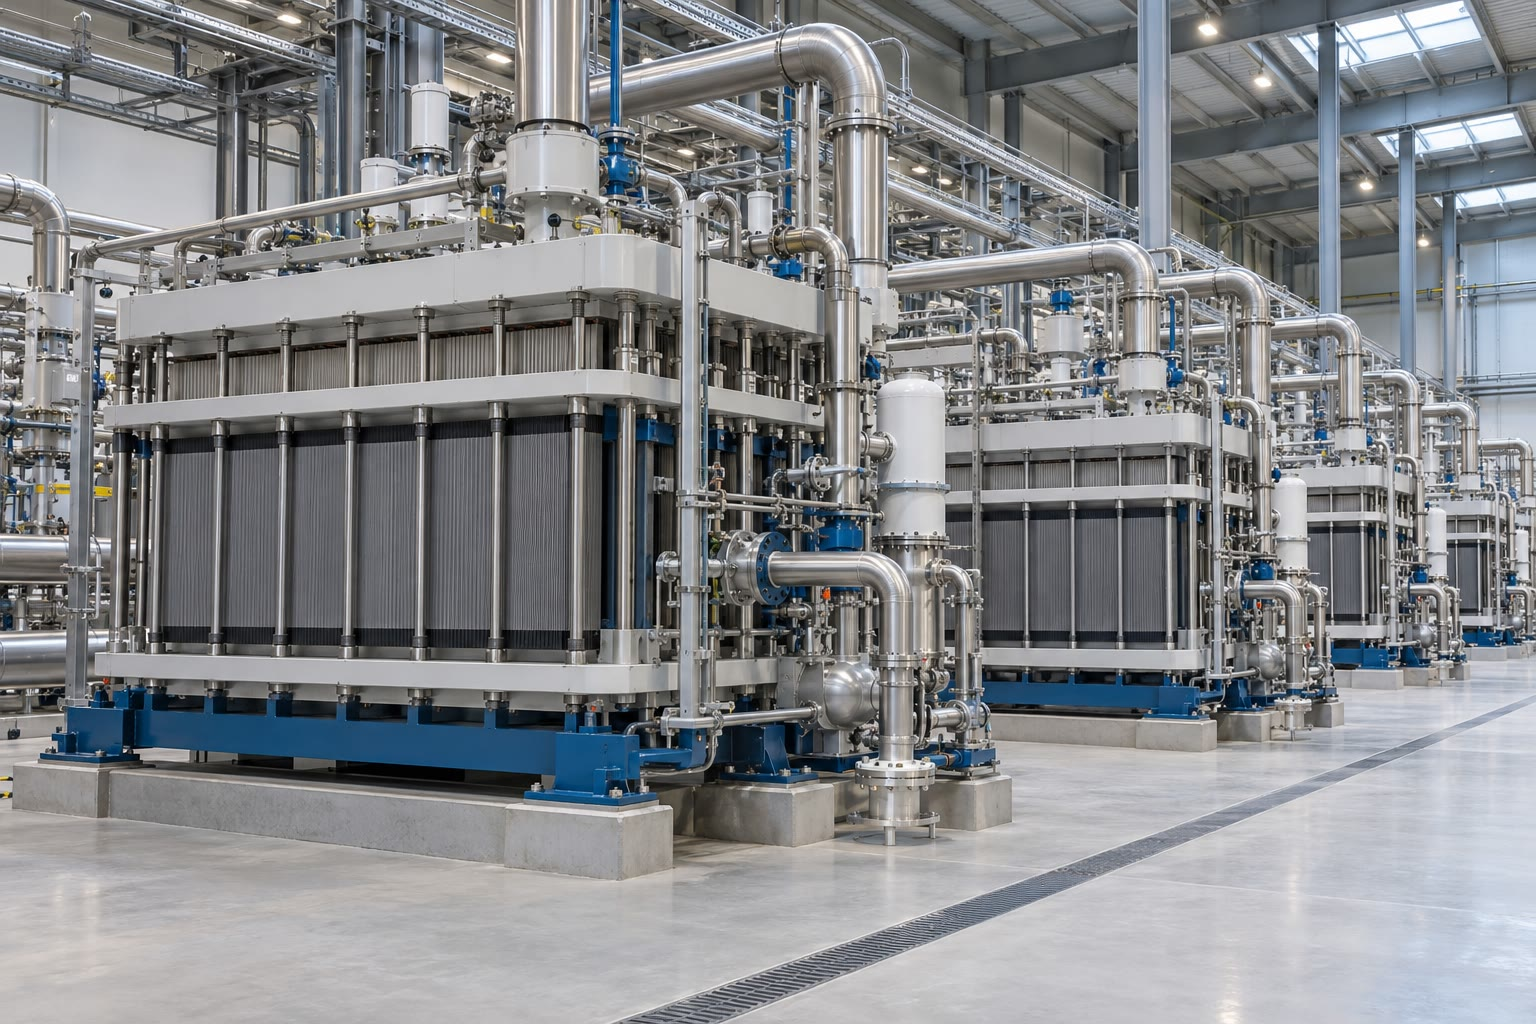
\includegraphics[width=0.48\linewidth]{images/book1/ai/g12-electrolyser-hall.jpg}

{\small قاعة محلّلات كهربائية: يُشطر الماء إلى ثنائي الهيدروجين
وثنائي الأكسجين.}
\end{omfigure}

\section{تمارين}

\begin{exercise}[$\star$]\label{exo:g12:cells-and-electrolysis:1}
في خلية دانيال، أي القطبين هو \omterm{def:g12:cells-and-electrolysis:anode}{المصعد}؟ وأيهما \omterm{def:g12:cells-and-electrolysis:anode}{المهبط}؟ اكتب
\omterm{def:g11:redox:couple}{نصف المعادلة} عند كل منهما.
\end{exercise}

\begin{exercise}[$\star$]\label{exo:g12:cells-and-electrolysis:2}
يسري تيار شدته \qty{0.20}{A} مدة \qty{30}{min}. احسب الشحنة
المنقولة وكمية \omterm{def:g9:inside-the-atom:nucleus}{الإلكترونات}.
\end{exercise}

\begin{exercise}[$\star$]\label{exo:g12:cells-and-electrolysis:3}
ما دور \omterm{def:g12:cells-and-electrolysis:cell}{الجسر الملحي}؟ وماذا يحدث إذا نُزع؟
\end{exercise}

\begin{exercise}[$\star$]\label{exo:g12:cells-and-electrolysis:4}
حوّل \omterm{def:g12:cells-and-electrolysis:capacity}{سعة} قدرها \qty{2.5}{A.h} إلى كولوم.
\end{exercise}

\begin{exercise}[$\star$]\label{exo:g12:cells-and-electrolysis:5}
في \omterm{def:g12:cells-and-electrolysis:electrolysis}{التحليل الكهربائي}، أيكون التفاعل تلقائيًا؟ وما الذي يمد
بالطاقة؟
\end{exercise}

\begin{exercise}[$\star\star$]\label{exo:g12:cells-and-electrolysis:6}
تتكوّن خلية من قطب فضة في نترات الفضة وقطب نحاس
في كبريتات النحاس. ويبيّن مقياس الفولت أن \omterm{def:g9:inside-the-atom:nucleus}{الإلكترونات} تغادر
من النحاس. اكتب نصفي المعادلتين، وسمِّ \omterm{def:g12:cells-and-electrolysis:anode}{المصعد} \omterm{def:g12:cells-and-electrolysis:anode}{والمهبط}،
وأعطِ التفاعل الإجمالي.
\end{exercise}

\begin{exercise}[$\star\star$]\label{exo:g12:cells-and-electrolysis:7}
تولّد بطارية ساعة \qty{10}{\micro A} باستمرار مدة ثلاث سنوات.
فما سعتها بالوحدة \si{mA.h}؟
\end{exercise}

\begin{exercise}[$\star\star$]\label{exo:g12:cells-and-electrolysis:8}
تُطلى ملعقة بالفضة بتيار شدته \qty{0.50}{A} مدة
\qty{40}{min}، \ce{Ag+ + e- -> Ag}. ما كتلة الفضة المترسبة؟
\end{exercise}

\begin{exercise}[$\star\star$]\label{exo:g12:cells-and-electrolysis:9}
على شكل خلية دانيال، أعطِ اتجاه التيار في
السلك، والاتجاه الذي تتحرك فيه \omterm{def:g9:ions:ion}{أيونات} \ce{K+} و\ce{NO3-} في
الجسر.
\end{exercise}

\begin{exercise}[$\star\star$]\label{exo:g12:cells-and-electrolysis:10}
قارن بين الخلية \omterm{def:g12:cells-and-electrolysis:electrolysis}{والتحليل الكهربائي}: إشارة \omterm{def:g12:cells-and-electrolysis:anode}{المصعد}، واتجاه
التفاعل، وتحويل الطاقة.
\end{exercise}

\begin{exercise}[$\star\star$]\label{exo:g12:cells-and-electrolysis:11}
في \omterm{def:g12:cells-and-electrolysis:electrolysis}{التحليل الكهربائي} للماء، يُجمع \qty{24}{mL} من ثنائي الهيدروجين.
فما حجم ثنائي الأكسجين المجموع في الوقت نفسه؟ ولماذا؟
\end{exercise}

\begin{exercise}[$\star\star\star$]\label{exo:g12:cells-and-electrolysis:12}
تحوي خلية دانيال \qty{5.0}{g} من الخارصين و\qty{100}{mL} من كبريتات
النحاس بتركيز \qty{0.50}{mol/L}. أي المتفاعلين ينفد أولًا؟ وما
\omterm{def:g12:cells-and-electrolysis:capacity}{سعة} الخلية؟ وكم من الوقت تستطيع توليد \qty{50}{mA}؟
\end{exercise}

\begin{exercise}[$\star\star\star$]\label{exo:g12:cells-and-electrolysis:13}
بطارية جهدها \qty{1.5}{V} توفر \qty{2.0}{A.h}. احسب الطاقة التي
تخزنها ($E = Q U$)، بالجول وبالواط ساعة.
\end{exercise}

\begin{exercise}[$\star\star\star$]\label{exo:g12:cells-and-electrolysis:14}
يُحلَّل الماء كهربائيًا بتيار \qty{2.0}{A} مدة \qty{1.0}{h}. احسب
كميتي ثنائي الهيدروجين وثنائي الأكسجين الناتجتين، ثم حجميهما عند \qty{20}{\celsius} ($V_m = \qty{24.1}{L/mol}$).
\end{exercise}

\begin{exercise}[$\star\star\star$]\label{exo:g12:cells-and-electrolysis:15}
في تنقية النحاس، يفقد \omterm{def:g12:cells-and-electrolysis:anode}{المصعد} \qty{3.00}{kg} من المادة بينما
يكسب \omterm{def:g12:cells-and-electrolysis:anode}{المهبط} \qty{2.84}{kg} من النحاس. ما النسبة المئوية للنحاس
في \omterm{def:g12:cells-and-electrolysis:anode}{المصعد} غير النقي، على افتراض أن النحاس وحده يتأكسد عند \omterm{def:g12:cells-and-electrolysis:anode}{المصعد}
وأن الشوائب تسقط فحسب؟
\end{exercise}

\section{مسألة: بطارية الهاتف}

\begin{problem}[{مسألة نهاية الأسبوع --- ما كتلة الليثيوم التي تتنقل بين
قطبي بطارية هاتف سعتها \qty{4000}{mA.h}؟}]
\label{pb:g12:cells-and-electrolysis:1}
% ledger: const:F, const:NA, aw:Li, dch:CH4, aw:C, aw:H
تحمل بطارية هاتف لصاقة «\qty{3.7}{V}، \qty{4000}{mA.h}». وفي صورة
مبسطة، تعطي كل \omterm{def:g7:atoms-and-molecules:atom}{ذرة} ليثيوم مخزنة في قطب الغرافيت إلكترونًا واحدًا أثناء
التفريغ وتغادر أيونَ ليثيوم،
\ce{Li -> Li+ + e-}؛ فيعبر \omterm{def:g9:ions:ion}{الأيون} الإلكتروليت ويستقبله
قطب الأكسيد الفلزي، الذي يكتسب إلكترونًا في الوقت نفسه.

\medskip
\noindent\textbf{الجزء الأول --- الخلية.}
\begin{enumerate}
  \item أثناء التفريغ، هل قطب الغرافيت هو \omterm{def:g12:cells-and-electrolysis:anode}{المصعد} أم
        \omterm{def:g12:cells-and-electrolysis:anode}{المهبط}؟ ولماذا؟
  \item أي القطبين هو السالب؟
  \item في أي اتجاه تنتقل \omterm{def:g9:inside-the-atom:nucleus}{الإلكترونات} عبر الهاتف؟
        \omterm{def:g9:ions:ion}{وأيونات} الليثيوم داخل البطارية؟
  \item لماذا تُعد هذه الخلية مركمًا؟
\end{enumerate}

\medskip
\noindent\textbf{الجزء الثاني --- الشحنة.}
\begin{enumerate}[resume]
  \item حوّل \qty{4000}{mA.h} إلى أمبير ساعة، ثم إلى كولوم.
  \item احسب كمية \omterm{def:g9:inside-the-atom:nucleus}{الإلكترونات} التي تمثلها هذه الشحنة.
  \item كم إلكترونًا يمثل ذلك؟
  \item يستهلك الهاتف في المتوسط \qty{0.25}{A}. فكم تدوم
        البطارية الممتلئة؟
  \item تُظهر الشاشة 20 \%. فما الشحنة الباقية بالكولوم؟
\end{enumerate}

\medskip
\noindent\textbf{الجزء الثالث --- الطاقة.}
\begin{enumerate}[resume]
  \item احسب الطاقة المخزنة، $E = Q U$، بالجول.
  \item حوّلها إلى واط ساعة.
  \item قارنها بالطاقة التي يطلقها حرق \qty{1}{g} من الميثان
        (\qty{55.7}{kJ}).
  \item كم شحنة كاملة يعطي \qty{1}{kW.h} من الكهرباء، لو
        لم تضع أي طاقة؟
\end{enumerate}

\medskip
\noindent\textbf{الجزء الرابع --- إعادة الشحن.}
\begin{enumerate}[resume]
  \item أثناء الشحن، أي تفاعل يجري عند قطب
        الغرافيت؟ أهو \omterm{def:g11:redox:oxidation}{أكسدة} أم \omterm{def:g11:redox:oxidation}{اختزال}؟
  \item لماذا تُعد إعادة الشحن تحليلًا كهربائيًا؟
  \item يوفر الشاحن \qty{2.0}{A}. فكم تستغرق إعادة الشحن الكاملة
        على الأقل؟
  \item ما كمية \omterm{def:g9:ions:ion}{أيونات} الليثيوم التي تعبر الإلكتروليت خلال
        شحنة كاملة واحدة؟
  \item احسب كتلتها.
  \item اذكر الجواب النهائي: ما كتلة الليثيوم التي تتنقل بين
        القطبين في شحنة كاملة واحدة؟
\end{enumerate}
\end{problem}
